\chapter{Systemmodelle}
\section{Anwendungsfälle}
\subsection{Bedienung der Android App}
\begin{center}
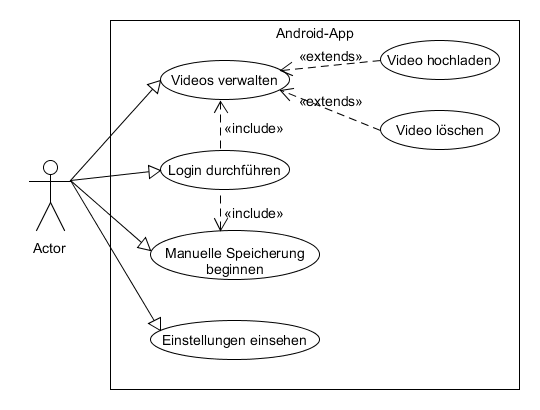
\includegraphics[width=1\textwidth]{subtopicsFuncspec/Res/systemModels/App-AFD-UML.png}
\end{center}
Dieser Anwendungsfall beschreibt die Bedienung der \gls{App}. 
Der Benutzer kann hierbei mehrere Aktionen ausführen:
\begin{itemize}
\itemsep0pt
\item Login durchführen
\item Videos verwalten
\item manuelle Speicherung beginnen
\item Einstellungen einsehen
\end{itemize}
Um die \gls{App} zu nutzen, muss sich der Benutzer zunächst auf der \gls{App} einloggen. Nach dem Einloggen kann der Benutzer sein aufgenommenes Videomaterial verwalten. Er kann z.B. Videos löschen oder an den \gls{Web-Dienst} senden.
Ist er in der Beobachtungsansicht, so ist es dem Nutzer möglich, die manuelle Speicherung des Videomaterials zu iniziieren. Außerdem ist es dem Benutzer möglich, die aufnahmespezifischen Einstellungen einzusehen.

\subsection{Bedienung der Website}
\begin{center}
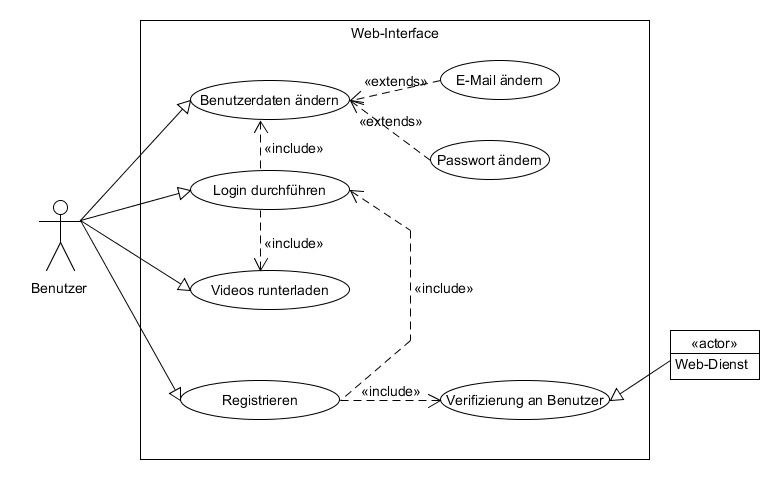
\includegraphics[width=1\textwidth]{subtopicsFuncspec/Res/systemModels/WebsiteAWFDiagram.png}
\end{center}	
Dieser Anwendungsfall beschreibt die Bedienung der Website.
Der Benutzer kann hierbei mehrere Aktionen ausführen:
\begin{itemize}
\itemsep0pt
\item Anmelden
\item Registrieren
\item Benutzerdaten ändern
\item Videos herunterladen
\end{itemize}
Um die Website zu nutzen, muss sich der Benutzer zunächst registrieren. Nach der Registrierung schickt der \gls{Web-Dienst} eine Verifizierungs-\gls{E-Mail} an den Benutzer. Nach der Bestätigung kann er sich auf der Webseite anmelden, um deren Funktionen zu nutzen. Ist der Benutzer eingeloggt, kann er seine Benutzerdaten ändern und zuvor hochgeladene, nun anonymisierte Videodaten herunterladen.

\section{Aktivitätsdiagramm}
\subsection{Vom Appstart bis zur Videofreigabe}
\begin{center}
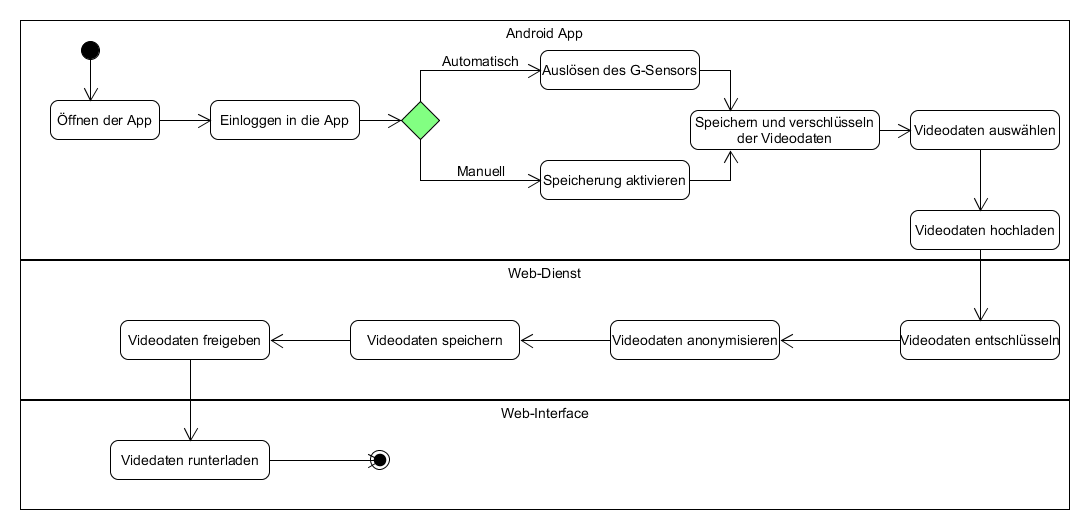
\includegraphics[width=1\textwidth]{subtopicsFuncspec/Res/systemModels/AKDiagramm.png}
\end{center}
Dieses Aktivitätsdiagramm beschreibt den Ablauf vom Start der \gls{App}, bis zur Freigabe und dem Herunterladen der Videodaten. 
\begin{enumerate}
\itemsep0pt
\item Öffnen der \gls{App}
\item Anmelden in der \gls{App}
\begin{description}
\item Der Benutzer meldet sich mit seinen Anmeldedaten in der \gls{App} an um die Funktionen zu nutzen.
\end{description}
\item Speicherung beginnen
\begin{enumerate}
\item Durch \gls{G-Sensor}
\begin{description}
\item Die vom \gls{G-Sensor} gemessene Beschleunigung ist größer als der festgelegte Richtwert.
\end{description}
\item Manuell
\begin{description}
\item Der Benutzer fordert manuell die Speicherung an.
\end{description}
\end{enumerate}
\item Speichern und verschlüsseln der Videodaten
\begin{description}
\item Nach Beendigung der Aufnahme werden die Videodaten verschlüsselt und daraufhin auf dem Smartphone gespeichert.
\end{description}
\item Videodaten auswählen
\item Videodaten hochladen
\begin{description}
\item Die ausgewählten Videodaten werden an den \gls{Web-Dienst} gesendet.
\end{description}
\item Videodaten entschlüsseln
\item Videodaten \gls{anonymisieren}
\begin{description}
\item Nach der Entschlüsselung der Videodaten anonymisiert der \gls{Web-Dienst} diese.
\end{description}
\item Videodaten speichern
\item Videodaten freigeben
\begin{description}
\item Die Videodaten werden dem Benutzer über das \gls{Web-Interface} zugänglich gemacht.
\end{description}
\item Videodaten herunterladen
\begin{description}
\item Nun kann der Benutzer sich einloggen und die anonymisierten Videodaten herunterladen.
\end{description}
\end{enumerate}